\part{13/1}

\section{Wiederholung}
\begin{itemize}
  \item relative Häufigkeit: Aussage über ein schon durchgeführtes Zufallsexperiment
  \item Wahrscheinlichkeit: Aussage über zukünftige Zufallsversuche
\end{itemize}
\begin{exercise}{456/5}
  \begin{gather*}
    F = \{(1, 1), (2, 1), (3, 1), (4, 1)\}
  \end{gather*}
  \item [a]
  \begin{gather*}
    E = \{(1, 1), (1, 2), (2, 1)\} \\\\
    F \colon \text{Die zweite Kugel trägt eine $1$} \\
    E \Leftrightarrow \text{Die Summe der Zahlen ist größer als $3$} \\\\
    P(E) = (\frac{2}{6} \cdot \frac{2}{6}) + (\frac{2}{6} \cdot \frac{1}{6}) + (\frac{1}{6} \cdot \frac{2}{6}) = \frac{2}{9} = 0.\overline{2} \\
    P(F) = (\frac{2}{6} \cdot \frac{2}{6}) + (\frac{1}{6} \cdot \frac{2}{6}) + (\frac{2}{6} \cdot \frac{2}{6}) + (\frac{1}{6} \cdot \frac{2}{6}) = P(1) = \frac{2}{6} = \frac{1}{3} = 0.\overline{3}
  \end{gather*}
  \item [b]
  \begin{gather*}
    E \cap F = \{(1, 1), (2, 1)\} \\
    P(E \cap F) = (\frac{2}{6} \cdot \frac{2}{6}) + (\frac{1}{6} \cdot \frac{2}{6}) = \frac{1}{6} = 0.1\overline{6}
  \end{gather*}
  \item [c]
  \begin{gather*}
    E \cup F = \{(1, 1), (1, 2), (2, 1), (3, 1), (4, 1)\} \\
    P(E \cup F) = (\frac{2}{6} \cdot \frac{2}{6}) + (\frac{2}{6} \cdot \frac{1}{6}) + (\frac{1}{6} \cdot \frac{2}{6}) + (\frac{2}{6} \cdot \frac{2}{6}) + (\frac{1}{6} \cdot \frac{2}{6}) = \frac{7}{18} = 0.3\overline{8}
  \end{gather*}
\end{exercise}
\begin{exercise}{456/7}
  \item [a]
  \begin{gather*}
    \text{Gegenwahrscheinlichkeit (keine Sechs werfen): } P(\neg E) = (\frac{5}{6})^5 \approx 0.40 \\
    P(E) = 1 - P(\neg E) = 1 - (\frac{5}{6})^5 \approx 0.60
  \end{gather*}
  \item [b]
  \begin{gather*}
    P = \frac{6}{6} \cdot \frac{5}{6} \cdot \frac{4}{6} \cdot \frac{3}{6} \cdot \frac{2}{6} = \approx 0.09
  \end{gather*}
  \item [c]
  \begin{gather*}
    P = (\frac{5}{6})^4 \cdot \frac{1}{6} \approx 0.08
  \end{gather*}
\end{exercise}
\begin{exercise}{456/9}
  \item [a]
  \begin{gather*}
    P = \frac{1}{13983816} \approx 7.15 \cdot 10^{-8}
  \end{gather*} \\\\
  Bemerkung: Ein Zufallsversuch heißt Laplace-Versuch, wenn alle Ergebnisse gleich wahrscheinlich sind.
  \begin{gather*}
    S = \{e_1, e_2, ..., e_n\} \qquad |S| = n \qquad P(e_i) = \frac{1}{n} \\
    E = \{e_1, ...\} \qquad |E| = k \qquad P(E) = \frac{k}{n}
  \end{gather*}
  $\Rightarrow$ Gleichverteilung
  \item [b]
  \begin{gather*}
    E = \{(1,2,3,4,5,6), (2,3,4,5,6,7), ..., (44,45,46,47,48,49)\} \\
    |E| = 44 \\
    P(E) = \frac{|E|}{|S|} = \frac{44}{13983816} \approx 3.15 \cdot 10^{-6}
  \end{gather*}
  \item [c]
  \begin{gather*}
    P = \frac{43}{49} \cdot \frac{42}{48} \cdot \frac{41}{47} \cdot \frac{40}{46} \cdot \frac{39}{45} \cdot \frac{38}{44} \approx 0.436
  \end{gather*}
\end{exercise}
\begin{exercise}{456/10}
  \item [a]
  \begin{gather*}
    \text{Anteil nach $10$ Tagen: } 0.85^{10} \approx 0.197 \\
    0.85^t = 0.5 \quad\Rightarrow\quad t = log_{0.85}(0.5) \approx 4.265
  \end{gather*}
  \item [b]
  \begin{gather*}
    (1 - p)^8 = 0.5 \quad\Rightarrow\quad p = 1 - \sqrt[8]{(0.5)} \approx 0.083
  \end{gather*}
\end{exercise}
\section{Abzählverfahren}
Bis auf Weiteres gilt: Die Zufallsversuche sind Laplace-Versuche. \\
Anzahl der Ergebnisse $N \quad\Rightarrow\quad P = \frac{1}{N} \quad\text{(Ergebniswahrscheinlichkeit)}$ \\\\
Ziehe $k$ mal aus einer Urne mit $n$ unterscheidbaren Kugeln:
\begin{itemize}
  \item mit Zurücklegen, unter Beachtung der Reihenfolge
  \begin{gather*}
    N = n^k
  \end{gather*}
  \item ohne Zurücklegen, unter Beachtung der Reihenfolge
  \begin{gather*}
    N = n \cdot (n - 1) \cdot (n - 2) \cdot ... \cdot \underbrace{(n - k + 1)}_{\mathclap{\text{übrige Kugeln vor dem $k$-ten Zug}}} = \frac{n!}{(n - k)!}
  \end{gather*}
  \item ohne Zurücklegen, ohne Beachtung der Reihenfolge \\\\
  Es werden jeweils $k!$ (Permutationen) Ergebnisse zu einem Ereignis zusammengefasst:
  \begin{gather*}
    N = \frac{n!}{(n - k)! \cdot k!} = \begin{pmatrix}n \\ k\end{pmatrix} \text{ (Binomialkoeffizient)}
  \end{gather*} \\
  Die Wahrscheinlichkeit für einen 6er im Lotto:
  \begin{gather*}
    p = \frac{1}{\begin{pmatrix}49 \\ 6\end{pmatrix}} \approx \frac{1}{14000000}
  \end{gather*}
  Die Wahrscheinlichkeit für einen 4er im Lotto (``Lottoproblem''):
  \begin{gather*}
    p = \frac{\begin{pmatrix}6 \\ 4\end{pmatrix} \cdot \begin{pmatrix}43 \\ 2\end{pmatrix}}{\begin{pmatrix}49 \\ 6\end{pmatrix}} = \frac{13545}{\begin{pmatrix}49 \\ 6\end{pmatrix}} \approx \frac{1}{1000}
  \end{gather*}
  \qquad (Wähle $4$ aus den $6$ Richtigen und $2$ aus den $43$ Falschen)
\end{itemize}
\begin{exercise}{460/1}
  \item [a]
  \begin{gather*}
    n = 2 \quad k = 6 \quad N = 2^6 = 64
  \end{gather*}
  \item [b]
  \begin{gather*}
    n = 4 \quad k = 4 \quad N = \frac{4!}{(4 - 4)!} = 4! = 24
  \end{gather*}
  \item [c]
  \begin{gather*}
    n = 3 \quad k = 5 \quad N = 3^5 = 243
  \end{gather*}
  \item [d]
  \begin{gather*}
    n = 10 \quad k = 2 \quad N = \begin{pmatrix}10 \\ 2\end{pmatrix} = 45
  \end{gather*}
\end{exercise}
\begin{exercise}{460/2}
  \item [a]
  \begin{gather*}
    n = 4 \quad k = 4 \quad N = 4^4 = 256
  \end{gather*}
  \item [b]
  \begin{gather*}
    p_1 = \frac{1}{2} \cdot \frac{1}{4} \cdot \frac{1}{8} \cdot \frac{1}{8} = \frac{1}{512} \\
    p_2 = \frac{4!}{p_1} = \frac{3}{64} \\
    p_3 = 1 - (\frac{1}{2})^4 = \frac{15}{16}
  \end{gather*}
\end{exercise}
\begin{exercise}{460/3}
  \item [a] Die Reihenfolge der Ziffern entspricht der Reihenfolge der Spiele.
  \item [b]
  \begin{gather*}
    p = (\frac{1}{3})^{11} = \frac{1}{177147} \approx 5.65 \cdot 10^{-6}
  \end{gather*}
  Annahme: Heimsieg, Gastsieg und Unentschieden sind jeweils gleich wahrscheinlich.
  \item [c]
  \begin{gather*}
    N = (\frac{2}{3})^{11} \cdot 3^{11} = 2^{11} = 2048
  \end{gather*}
\end{exercise}
\begin{exercise}{460/5}
  \begin{gather*}
    N = \frac{12!}{(12 - 3)!} = 1320
  \end{gather*}
\end{exercise}
\begin{exercise}{461/8}
  \item [a]
  \begin{gather*}
    N = 5! = 120
  \end{gather*}
  \item [b]
  \begin{gather*}
    p = \frac{1}{5}
  \end{gather*}
  \item [c]
  \begin{gather*}
    \frac{1}{5} \cdot \frac{1}{4} = \frac{1}{20}
  \end{gather*}
\end{exercise}
\begin{exercise}{461/11}
  \item [a]
  \begin{gather*}
    p = \frac{6}{49} \cdot \frac{5}{48} \cdot \frac{4}{47} \cdot \frac{3}{46} \cdot \frac{43}{45} \cdot \frac{42}{44} \approx 6.46 \cdot 10^{-5}
  \end{gather*}
  \item [b]
  \begin{gather*}
    rrrrff, rrrfrf, rrfrrf, rfrrrf, frrrrf, \\
    rrrffr, rrfrfr, rfrrfr, frrrfr, \\
    rrffrr, rfrfrr, frrfrr, \\
    rffrrr, frfrrr, \\
    ffrrrr
  \end{gather*}
  \item [c]
  \begin{gather*}
    p_4 \approx 15 \cdot 6.46 \cdot 10^{-5} \approx 9.69 \cdot 10^{-4}
  \end{gather*}
  \item [d]
  \begin{gather*}
    p_2 = \begin{pmatrix}6 \\ 2\end{pmatrix} \cdot (\frac{6}{49} \cdot \frac{5}{48} \cdot \frac{43}{47} \cdot \frac{42}{46} \cdot \frac{41}{45} \cdot \frac{40}{44}) \approx 0.13
  \end{gather*}
  \item [e]
  \begin{gather*}
    p_0 = \begin{pmatrix}6 \\ 0\end{pmatrix} \cdot (\frac{43}{49} \cdot \frac{42}{48} \cdot \frac{41}{47} \cdot \frac{40}{46} \cdot \frac{39}{45} \cdot \frac{38}{44}) \approx 0.44 \\
    p_1 = \begin{pmatrix}6 \\ 1\end{pmatrix} \cdot (\frac{6}{49} \cdot \frac{43}{48} \cdot \frac{42}{47} \cdot \frac{41}{46} \cdot \frac{40}{45} \cdot \frac{39}{44}) \approx 0.41 \\
    p_{\geq 3} = 1 - (p_0 + p_1 + p_2) \approx 1.86 \cdot 10^{-2} \\\\
    p_{50Sp.} = 1 - (p_0 + p_1 + p_2)^{50} \approx 0.61 \\
    p_{100Sp.} = 1 - (p_0 + p_1 + p_2)^{100} \approx 0.85 \\
    p_{1000Sp.} = 1 - (p_0 + p_1 + p_2)^{1000} \approx 1.00
  \end{gather*}
\end{exercise}
\begin{exercise}{461/10}
  \item [a]
  \begin{gather*}
    p = \begin{pmatrix}6 \\ 6\end{pmatrix} \cdot (\frac{6}{45} \cdot \frac{5}{44} \cdot \frac{4}{43} \cdot \frac{3}{42} \cdot \frac{2}{41} \cdot \frac{1}{40}) = \frac{1}{\begin{pmatrix}45 \\ 6\end{pmatrix}} \approx 1.23 \cdot 10^{-7}
  \end{gather*}
  \item [b]
  \begin{gather*}
    N = \begin{pmatrix}5 \\ 2\end{pmatrix} = 10
  \end{gather*}
  \item [c]
  \begin{gather*}
    N = \begin{pmatrix}1000 \\ 2\end{pmatrix} = 4.995 \cdot 10^{5}
  \end{gather*}
\end{exercise}
\subsubsection{AB Grundbegriffe der Wahrscheinlichkeitsrechnung}
\begin{exercise}{AB/12}
  \begin{gather*}
    p = \frac{6}{7} \cdot \frac{4}{5} \cdot \frac{2}{3} \approx 0.46
  \end{gather*}
\end{exercise}
\begin{exercise}{AB/17}
  \item [a]
  \begin{gather*}
    N = \begin{pmatrix}16 \\ 3\end{pmatrix} \cdot \begin{pmatrix}8 \\ 2\end{pmatrix} = 39200
  \end{gather*}
  \item [b]
  \begin{gather*}
    N = \begin{pmatrix}24 \\ 5\end{pmatrix} - \begin{pmatrix}16 \\ 5\end{pmatrix} = 38136
  \end{gather*}
\end{exercise}
\begin{exercise}{AB/20}
  \begin{gather*}
    p_{3r} = \frac{\begin{pmatrix}5 \\ 3\end{pmatrix} \cdot \begin{pmatrix}15 \\ 5\end{pmatrix}}{\begin{pmatrix}20 \\ 8\end{pmatrix}} \approx 0.2384 \\
    p_{\geq 4r} = \frac{\begin{pmatrix}5 \\ 4\end{pmatrix} \cdot \begin{pmatrix}15 \\ 4\end{pmatrix}}{\begin{pmatrix}20 \\ 8\end{pmatrix}} + \frac{\begin{pmatrix}5 \\ 5\end{pmatrix} \cdot \begin{pmatrix}15 \\ 3\end{pmatrix}}{\begin{pmatrix}20 \\ 8\end{pmatrix}} \approx 0.0578
  \end{gather*}
\end{exercise}
\begin{exercise}{AB/21}
  \begin{gather*}
    p_2 = \frac{\begin{pmatrix}10 \\ 2\end{pmatrix} \cdot \begin{pmatrix}90 \\ 3\end{pmatrix}}{\begin{pmatrix}100 \\ 5\end{pmatrix}} \approx 0.0702 \\\\
    p_{\geq 3} = p_3 + p_4 + p_5 \\
    \;= \frac{\begin{pmatrix}10 \\ 3\end{pmatrix} \cdot \begin{pmatrix}90 \\ 2\end{pmatrix} + \begin{pmatrix}10 \\ 4\end{pmatrix} \cdot \begin{pmatrix}90 \\ 1\end{pmatrix} + \begin{pmatrix}10 \\ 5\end{pmatrix} \cdot \begin{pmatrix}90 \\ 0\end{pmatrix}}{\begin{pmatrix}100 \\ 5\end{pmatrix}} \approx 0.0066
  \end{gather*}
\end{exercise}
\begin{exercise}{AB/11}
  \item [a]
  \begin{gather*}
    N = (4 + 5 + 3)! = 479001600
  \end{gather*}
  \item [b]
  \begin{gather*}
    N = 3! \cdot 4! \cdot 5! \cdot 3! = 103680
  \end{gather*}
\end{exercise}
\begin{exercise}{AB/13}
  \begin{gather*}
    t = \frac{26!}{10^6} \approx 4.0329 \cdot 10^{20}ms \approx 1.2780 \cdot 10^{10}y \approx 0.93 \cdot \text{Alter des Universums}
  \end{gather*}
\end{exercise}
\begin{exercise}{AB/23}
  \begin{gather*}
    p_3 = \frac{\begin{pmatrix}4 \\ 3\end{pmatrix} \cdot \begin{pmatrix}12 \\ 1\end{pmatrix}}{\begin{pmatrix}16 \\ 4\end{pmatrix}} \approx 2.6374 \cdot 10^{-2} \\
    p_4 = \frac{\begin{pmatrix}4 \\ 4\end{pmatrix} \cdot \begin{pmatrix}12 \\ 0\end{pmatrix}}{\begin{pmatrix}16 \\ 4\end{pmatrix}} \approx 5.4945 \cdot 10^{-4} \\
    Erw = 1 - (10 \cdot p_3 + 1000 \cdot p_4) \approx 0.19
  \end{gather*}
\end{exercise}
\section{Bedingte Wahrscheinlichkeit}
Aus einer Urne mit $6$ roten und $4$ blauen Kugeln werden $2$ Kugeln ohne Zurücklegen gezogen.
\begin{gather*}
  \begin{tikzpicture}[grow=down]
    \tikzstyle{level 1} = [level distance=2.5cm, sibling distance=6cm]
    \tikzstyle{level 2} = [level distance=2.5cm, sibling distance=3cm]
    \tikzstyle{level 3} = [level distance=2.5cm, sibling distance=1.5cm]
    \node {1. Zug}
      child {
        node {2. Zug}
        child {
          node {$({\color{blue}b}, {\color{blue}b})$}
          edge from parent
          node[above left] {\color{blue}$\frac{3}{9}$}
        }
        child {
          node {$({\color{blue}b}, {\color{red}r})$}
          edge from parent
          node[above right] {\color{red}$\frac{6}{9}$}
        }
        edge from parent
        node[above left] {\color{blue}$\frac{4}{10}$}
      }
      child {
        node {2. Zug}
        child {
          node {$({\color{red}r}, {\color{blue}b})$}
          edge from parent
          node[above left] {\color{blue}$\frac{4}{9}$}
        }
        child {
          node {$({\color{red}r}, {\color{red}r})$}
          edge from parent
          node[above right] {\color{red}$\frac{5}{9}$}
        }
        edge from parent
        node[above right] {\color{red}$\frac{6}{10}$}
      };
    \end{tikzpicture}
\end{gather*}
\begin{gather*}
  E \colon \text{rot im ersten Zug} \qquad P(E) = \frac{6}{10} \\
  F \colon \text{rot im zweiten Zug} \qquad P(F) = \frac{4}{10} \cdot \frac{6}{9} + \frac{6}{10} \cdot \frac{5}{9} = \frac{3}{5} \\\\
  P_E(F) = \frac{5}{9} \qquad \text{Wahrscheinlichkeit für Ereignis $F$, unter der Voraussetzung,} \\
  \qquad\qquad\qquad\quad\text{dass Ereignis $E$ zurvor eingetreten ist}
\end{gather*}
\subsection{Statistische Unabhängigkeit}
Wenn gilt, dass $P_E(F) = P(F)$, dann sagt man die Ereignisse $E$ und $F$ sind statistisch unabhängig.
\begin{gather*}
  E \colon \text{rot im ersten Zug} \qquad P(E) = \frac{6}{10} \\
  F \colon \text{rot im zweiten Zug} \qquad P(F) = \frac{3}{5} \\\\
  P_E(F) = \frac{5}{9} \neq P(F) = \frac{3}{5}
\end{gather*}
Die Wahrscheinlichkeit, dass rot im zweiten Zug gezogen wird unter der Bedingung, dass rot schon im ersten Zug gezogen wurde, ist ungleich der Wahrscheinlichkeit, dass allgemein rot im zweiten Zug gezogen wird. \\
$E$ und $F$ sind statistisch abhängig. \\
\begin{gather*}
  \overline{E} \colon \text{blau im ersten Zug} \\
  \overline{F} \colon \text{blau im zweiten Zug} \\\\
  P_{\overline{E}}(F) = \frac{6}{9} \neq P(F) = \frac{3}{5} \\
  P_E(\overline{F}) = \frac{4}{9} \neq P(\overline{F}) = \frac{2}{5} \\
  P_{\overline{E}}(\overline{F}) = \frac{3}{9} \neq P(\overline{F}) = \frac{2}{5}
\end{gather*}
\begin{exercise}{475/1}
  \item [a]
  \begin{gather*}
    P = 0.98^4 \approx 0.9224
  \end{gather*}
  \item [b]
  Wenn bei einem Fahrzeug eine Panne auftritt, besteht die Möglichkeit, dass dies auf ein besonders anfälliges Fahrzeugteil oder einen Produktionsfehler zurückzuführen ist, welches/r sich auch in den anderen drei Fahrzeugen befindet.
\end{exercise}
\newpage
\begin{exercise}{475/2}
  \item [a]
  \begin{gather*}
    P(E) = \frac{3}{5} \qquad P(F) = \frac{2}{5} \\
    E \cap F = \{(a_1, h_1), (a_1, h_2), (a_2, h_1), ..., (a_3, h_2)\} \qquad |E \cap F| = 6 \\
    P(E \cap F) = \frac{|E \cap F|}{5^2} = P(E) \cdot P(F) = \frac{6}{25}
  \end{gather*}
  \item [b]
  \begin{gather*}
    P(E) = \frac{3}{5} \qquad P(F) = \frac{3}{5} \cdot \frac{2}{4} + \frac{2}{5} \cdot \frac{1}{4} = 0.34 \\
    P(E \cap F) = \frac{3}{5} \cdot \frac{2}{4} = 0.3 \neq P(E) \cdot P(F) = 0.204 \\
    P_E(F) = \frac{2}{4} = \frac{1}{2}
  \end{gather*}
\end{exercise}
\subsubsection{Vierfelder-Tafel}
\begin{gather*}
  E \colon \text{Raucher} \qquad \overline{E} \colon \text{Nichtraucher} \\
  F \colon \text{mit Gewicht zufrieden} \qquad \overline{F} \colon \text{mit Gewicht unzufrieden}
\end{gather*}
\begin{tabular}{c|c|c|c}
  & $F$ & $\overline{F}$ & \\ \hline
  $E$ & $P(E \cap F)$ & $P(E \cap \overline{F})$ & $P(E)$ \\ \hline
  $\overline{E}$ & $P(\overline{E} \cap F)$ & $P(\overline{E} \cap \overline{F})$ & $P(\overline{E})$ \\ \hline
  & $P(F)$ & $P(\overline{F})$ & $100\%$
\end{tabular}
\begin{gather*}
  P_E(F) = \frac{P(E \cap F)}{P(E)}
\end{gather*}
\begin{exercise}{476/11}
  \begin{gather*}
    P(\text{V. h.} \cap \text{S. h.}) = \frac{471}{1000} = 47.1\% \\
    P(\text{V. h}) \cdot P(\text{S. h.}) = \frac{622}{1000} \cdot \frac{619}{1000} \approx 38.5\% \\\\
    P(\text{V. h.} \cap \text{S. h.}) \neq P(\text{V. h}) \cdot P(\text{S. h.}) \quad\Rightarrow\quad \text{statistisch abhängig}
  \end{gather*}
\end{exercise}
\subsection{Der Satz von Bayes}
\begin{gather*}
  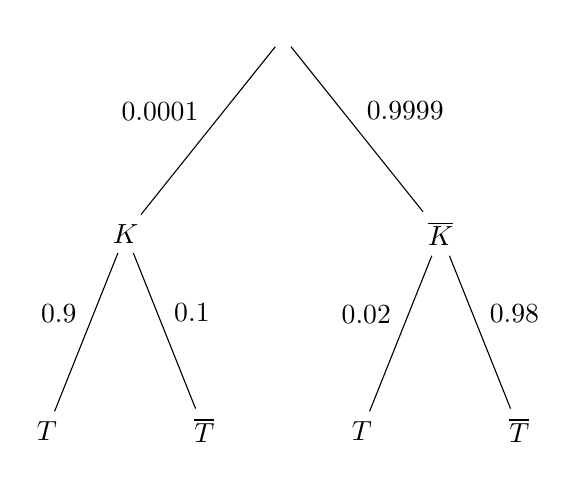
\begin{tikzpicture}[grow=down]
    \tikzstyle{level 1} = [level distance=2.5cm, sibling distance=4cm]
    \tikzstyle{level 2} = [level distance=2.5cm, sibling distance=2cm]
    \tikzstyle{level 3} = [level distance=2.5cm, sibling distance=1cm]
    \node {}
      child {
        node {$K$}
        child {
          node {$T$}
          edge from parent
          node[above left] {$0.9$}
        }
        child {
          node {$\overline{T}$}
          edge from parent
          node[above right] {$0.1$}
        }
        edge from parent
        node[above left] {$0.0001$}
      }
      child {
        node {$\overline{K}$}
        child {
          node {$T$}
          edge from parent
          node[above left] {$0.02$}
        }
        child {
          node {$\overline{T}$}
          edge from parent
          node[above right] {$0.98$}
        }
        edge from parent
        node[above right] {$0.9999$}
      };
    \end{tikzpicture}
\end{gather*}
\begin{gather*}
  P_K(T) = 0.90 \colon \text{Sensitivität des Tests} \\
  P_{\overline{K}}(\overline{T}) = 0.98 \colon \text{Spezifität des Tests} \\\\
  K \colon \text{krank} \qquad T \colon \text{positiver Test} \\
  P_T(K) \colon \text{Wahrscheinlichkeit, krank zu sein, wenn der Test positiv ausfällt} \\\\
  P_T(K) = \frac{P(K \cap T)}{P(T)} = \frac{P(K) \cdot P_K(T)}{P(K) \cdot P_K(T) + P(\overline{K}) \cdot P_{\overline{K}}(T)} \\\\
  P(K) \cdot P_K(T) = P(T) \cdot P_T(K) \\
  P(T) = P(K) \cdot P_K(T) + P(\overline{K}) \cdot P_{\overline{K}}(T) \\
  \; = 0.0001 \cdot 0.9 + 0.9999 \cdot 0.02 \\
  \;= 0.00009 + 0.02 \\
  \;= 0.02009
\end{gather*}
\begin{exercise}{479/2}
  \item [b]
  \begin{gather*}
    P_+(\text{krank}) = \frac{0.09}{0.1} = 90\%
  \end{gather*}
  \item [c]
  \begin{gather*}
    P_-(\text{gesund}) = \frac{0.89}{0.9} = 98.\overline{8}\%
  \end{gather*}
\end{exercise}
\begin{exercise}{479/3}
  \begin{gather*}
    P(A) = 0.4 \quad P(\text{einwandfrei}) = 0.95 \\
    P(A \cap \text{einwandfrei}) = 0.4 \cdot 0.9 = 0.36
  \end{gather*}
  \begin{tabular}{c|c|c|c}
    & $A$ & $\overline{A}$ & \\ \hline
    einwandfrei & $0.36$ & $0.95 - 0.36 = 0.59$ & $0.95$ \\ \hline
    defekt & $0.4 - 0.36 = 0.04$ & $0.05 - 0.04 = 0.01$ & $1 - 0.95 = 0.05$ \\ \hline
    & $0.4$ & $1 - 0.4 = 0.6$ & $100\%$
  \end{tabular}
  \begin{gather*}
    P_\text{defekt}(A) = \frac{0.04}{0.05} = 80\%
  \end{gather*}
\end{exercise}
\begin{exercise}{479/4}
  \begin{gather*}
    P(\text{Bahn}) = 0.8 \quad P(\text{pünktlich}) = 0.6 \\
    P_\text{Bahn}(\text{pünktlich}) = 0.\overline{6}
  \end{gather*}
  \begin{tabular}{c|c|c|c}
    & Bahn & nicht Bahn & \\ \hline
    pünktlich & $0.\overline{6} \cdot 0.8 = 0.5\overline{3}$ & $0.6 - 0.5\overline{3} = 0.0\overline{6}$ & $0.6$ \\ \hline
    unpünktlich & $0.8 - 0.5\overline{3} = 0.2\overline{6}$ & $0.2 - 0.0\overline{6} = 0.1\overline{3}$ & $1 - 0.6 = 0.4$ \\ \hline
    & $0.8$ & $1 - 0.8 = 0.2$ & $100\%$
  \end{tabular}
  \begin{gather*}
    P_\text{pünktlich}(\text{Bahn}) = \frac{0.5\overline{3}}{0.6} = 88.\overline{8}\%
  \end{gather*}
\end{exercise}
\begin{exercise}{479/5}
  \begin{gather*}
    P_{\text{krank}}(\text{negativ}) = 0.0001 \quad P_{\text{gesund}}(\text{positiv}) = 0.001 \\
    P(\text{krank}) = \frac{100}{1100000} = 0.000\overline{09}
  \end{gather*}
  \begin{tabular}{c|c|c|c}
    & krank & gesund & \\ \hline
    positiv & $9.09 \cdot 10^{-5}$ & $9.99\overline{90} \cdot 10^{-4}$ & $0.0010908\overline{09}$ \\ \hline
    negativ & $9.\overline{09} \cdot 10^{-9}$ & $0.998909\overline{18}$ & $0.989091\overline{09}$ \\ \hline
    & $0.000\overline{09}$ & $0.999\overline{90}$ & $100\%$
  \end{tabular}
  \begin{gather*}
    P_{\text{positiv}}(\text{krank}) = \frac{P(\text{krank} \cap \text{positiv})}{P(\text{positiv})} = \frac{9.09 \cdot 10^{-5}}{0.0010908\overline{09}} \approx 8.33\%
  \end{gather*}
\end{exercise}
\newpage
\begin{exercise}{479/6}
  \item [a]
  \begin{gather*}
    B_1 = \{w_1, w_2, s_1, ... s_5\} \qquad B_2 = \{w_1, ..., w_4, s_1, ..., s_4\} \\\\
    P(B_1) = P(B_2) = \frac{1}{2} \\
    P_{B_1}(w) = \frac{2}{7} \qquad P_{B_1}(s) = \frac{5}{7} \qquad P_{B_2}(w) = P_{B_2}(s) = \frac{1}{2} \\
    P(s) = P(B_1) \cdot P_{B_1}(s) + P(B_2) \cdot P_{B_2}(s) = \frac{17}{28} \\\\
    P_s(B_1) = \frac{P(B_1) \cdot P_{B_1}(s)}{P(s)} \approx 58.82\% \\
    P_s(B_2) = \frac{P(B_2) \cdot P_{B_2}(s)}{P(s)} \approx 41.18\%
  \end{gather*}
  \item [b]
  \begin{gather*}
    P_{B_1}((s, s)) = \frac{5}{7} \cdot \frac{4}{6} = \frac{10}{21} \qquad P_{B_2}((s, s)) = \frac{1}{2} \cdot \frac{3}{7} = \frac{3}{14} \\
    P((s, s)) = P(B_1) \cdot P_{B_1}((s, s)) + P(B_2) \cdot P_{B_2}((s, s)) = \frac{29}{84} \\\\
    P_{(s, s)}(B_1) = \frac{P(B_1) \cdot P_{B_1}(s, s)}{P(s, s)} \approx 68.97\% \\
    P_{(s, s)}(B_2) = \frac{P(B_2) \cdot P_{B_2}(s, s)}{P(s, s)} \approx 31.03\%
  \end{gather*}
\end{exercise}
\section{Zufallsgrößen - Erwartungswert, Standardabweichung}
Eine Zufallsgröße (eigentlich eine Funktion) weist jedem Element (Ergebnis) der Ergebnismenge $S$ eine Zahl oder einen Wert zu. \\\\
Beispiel: Losbude. Die Urne enthält $1000$ Lose, darunter $50$ Trostpreise (Wert $1.50€$), $5$ größere Preise (Wert $4€$) und $1$ Hauptgewinn (Wert $10€$). Jedes Los kostet $1€$. \\
Die Zufallsgröße $X$ hat vier Werte (Niete, Trostpreis, größerer Preis, Hauptgewinn) also $x_1$, $x_2$, $x_3$, $x_4$. Die Zufallsgröße zerlegt die Ergebnismenge vollständig und ohne Überlappung in Ereignisse. \\\\
Wahrscheinlichkeitsverteilung: Notiere zu jedem Wert, den eine Zufallsgröße annehmen kann, die Wahrscheinlichkeit
\begin{gather*}
  P(X = x_1) = \frac{944}{1000} \qquad P(X = x_2) = \frac{50}{1000} \\
  P(X = x_3) = \frac{5}{1000} \qquad P(X = x_4) = \frac{1}{1000}
\end{gather*}
Erwartungswert
\begin{gather*}
  \text{durchschnittlicher Bruttogewinn ohne Lospreis (Sicht des Spielers):} \\
  \mu = 0€ \cdot \frac{944}{1000} + 1.50€ \cdot \frac{50}{1000} + 4€ \cdot \frac{5}{1000} + 10€ \cdot \frac{1}{1000} = 0.105€ \\\\
  \text{durchschnittlicher Erlös, Nettogewinn inkl. Lospreis (Sicht der Losbude):} \\
  \mu = 1€ \cdot 1 - 0€ \cdot \frac{944}{1000} - 1.50€ \cdot \frac{50}{1000} - 4€ \cdot \frac{5}{1000} - 10€ \cdot \frac{1}{1000} = 0.895€ \\\\
  \text{allgemein:} \\
  \mu = P(X = x_1) \cdot x_1 + P(X = x_2) \cdot x_2 + ... = \sum_{i = 1}^n P(X = x_i) \cdot x_i
\end{gather*}
Standardabweichung (mittl. Schwankungsbreite um den Erwartungswert herum)
\begin{gather*}
  \sigma = \sqrt{P(X = x_1) \cdot (x_1 - \mu)^2 + P(X = x_2) \cdot (x_2 - \mu)^2 + ...} \\
  \;= \sqrt{\sum_{i = 1}^n P(X = x_2) \cdot (x_i - \mu)^2} \\
  \;= \sqrt{\frac{944}{1000} \cdot (-0.105€)^2 + \frac{50}{1000} \cdot (1.395€)^2 + \frac{5}{1000} \cdot (3.895€)^2 + \frac{1}{1000} \cdot (9.895€)^2} \\
  \;\approx 0.5305€
\end{gather*}
\begin{exercise}{488/1}
  \begin{gather*}
    \mu = \frac{1}{4} \cdot (-10) + \frac{1}{2} \cdot 5 + \frac{1}{12} \cdot 10 = \frac{5}{6} \\
    \sigma = \sqrt{\frac{1}{4} \cdot (-\frac{65}{6})^2 + \frac{1}{6} \cdot (-\frac{5}{6})^2 + \frac{1}{2} \cdot (\frac{25}{6})^2 + \frac{1}{12} \cdot (\frac{55}{6})^2} \approx 6.7185
  \end{gather*}
\end{exercise}
\begin{exercise}{488/2}
  \begin{gather*}
    P(X = 0) \approx 0.1176 \qquad P(X = 1) \approx 0.3674 \\
    P(X = 2) \approx 0.3823 \qquad P(X = 3) \approx 0.1327 \\\\
    \mu \approx 0.3674 \cdot 1 + 0.3823 \cdot 2 + 0.1327 \cdot 3 \approx 1.53 = 3 \cdot 0.51 \\
    \sigma \approx \sqrt{
      \begin{aligned}
        &0.1176 \cdot (-1.53)^2 + 0.3674 \cdot (-0.53)^2 \\
        &+ 0.3823 \cdot (0.47)^2 + 0.1327 \cdot (1.47)^2
      \end{aligned}
    } \approx 0.87
  \end{gather*}
\end{exercise}
\begin{exercise}{488/3}
  \begin{gather*}
    \mu = 0 \cdot 0.436 + 1 \cdot 0.413 + 2 \cdot 0.132 + 3 \cdot 0.0177 + 4 \cdot 0.000969 \\
    \;+ 5 \cdot 1.85 \cdot 10^{-5} + 6 \cdot 7.15 \cdot 10^{-8} \approx 0.7341 \\
    \sigma = \sqrt{(-0.7341)^2 \cdot 0.436 + ... + (5.2659)^2 \cdot 7.15 \cdot 10^{-8}} \approx 0.7598
  \end{gather*}
\end{exercise}
\begin{exercise}{488/4}
  \begin{gather*}
    P(X = 0.5 + 0.5 = 1) = \frac{12}{25} \cdot \frac{11}{24} = 0.22 \\
    P(X = 1 + 0.5 = 1.5) = \frac{5}{25} \cdot \frac{12}{24} + \frac{12}{25} \cdot \frac{5}{24} = 0.2 \\
    P(X = 1 + 1 = 2) = \frac{5}{25} \cdot \frac{4}{24} = 0.0\overline{3} \\
    P(X = 2 + 0.5 = 2.5) = \frac{8}{25} \cdot \frac{12}{24} + \frac{12}{25} \cdot \frac{8}{24} = 0.32 \\
    P(X = 2 + 1 = 3) = \frac{8}{25} \cdot \frac{5}{24} + \frac{5}{25} \cdot \frac{8}{24} = 0.1\overline{3} \\
    P(X = 2 + 2 = 4) = \frac{8}{25} \cdot \frac{7}{24} = 0.09\overline{3} \\\\
    m = \mu = 0.22 \cdot 1 + 0.2 \cdot 1.5 + 0.0\overline{3} \cdot 2 + 0.32 \cdot 2.5 + 0.1\overline{3} \cdot 3 + 0.09\overline{3} \cdot 4 \\
    \;= 2.16 \\
    \sigma = \sqrt{
      \begin{aligned}
        &0.22 \cdot (-1.16)^2 + 0.2 \cdot (-0.66)^2 + 0.0\overline{3} \cdot (-0.16)^2 \\
        &+ 0.32 \cdot (0.34)^2 + 0.1\overline{3} \cdot (0.84)^2 + 0.09\overline{3} \cdot (1.84)^2
      \end{aligned}
    } \approx 0.9116
  \end{gather*}
\end{exercise}
\begin{exercise}{489/10}
  \begin{gather*}
    P(X = 0) = 0.2^3 = 0.008 \qquad P(X = 1) = 3 \cdot 0.8 \cdot 0.2^2 = 0.096 \\
    P(X = 2) = 3 \cdot 0.8^2 \cdot 0.2 = 0.384 \qquad P(X = 3) = 0.8^3 = 0.512 \\\\
    \mu = 0 \cdot 0.008 + 1 \cdot 0.096 + 2 \cdot 0.384 + 3 \cdot 0.512 = 2.4 = 3 \cdot 0.8
  \end{gather*}
\end{exercise}
\begin{exercise}{489/11}
  \begin{gather*}
    P(X = 3) = \frac{1}{4} \qquad P(X = 4) = \frac{3}{8} \qquad P(X = 5) = \frac{3}{8} \\\\
    \mu = 3 \cdot \frac{1}{4} + 4 \cdot \frac{3}{8} + 5 \cdot \frac{3}{8} = 4.125 \\
    \sigma = \sqrt{(3 - 4.125)^2 \cdot \frac{1}{4} + (4 - 4.125)^2 \cdot \frac{3}{8} + (5 - 4.125)^2 \cdot \frac{3}{8}} \approx 0.781
  \end{gather*}
\end{exercise}
\section{Bernoulli-Experiment, Binomialverteilung}
Ein Bernoulli-Experiment hat $2$ Versuchsausgänge (Treffer, Niete).
$$P(\text{Treffer}) = p \qquad P(\text{Niete}) = q = 1 - p$$
Eine Folge von Bernoulli-Experimenten heißt Bernoulli-Kette. \\\\
Frage: Wie viele Treffer $k$ kommen bei einer Bernoulli-Kette der Länge $n$ vor? \\\\
Beispiel: Würfle $10$ mal; wie wahrscheinlich sind $3$ Sechser?
\begin{gather*}
  n = 10 \qquad p = \frac{1}{6} \qquad k = 3 \\
  P(\text{ein Pfad}) = (\frac{1}{6})^3 \cdot (\frac{5}{6})^7 \qquad \text{Anzahl der Pfade mit $3$ Treffern: } \begin{pmatrix}10 \\ 3\end{pmatrix} \\
  P(\text{$3$ Sechser, $10$ Würfe}) = (\frac{1}{6})^3 \cdot (\frac{5}{6})^7 \cdot \begin{pmatrix}10 \\ 3\end{pmatrix} \approx 0.1550
\end{gather*}
Allgemein gilt:
\begin{gather*}
  P(k, n, p) = p^k \cdot (1 - p)^{n - k} \cdot \begin{pmatrix}n \\ k\end{pmatrix}
\end{gather*}
Schreibweise:
\begin{gather*}
  P(k, n, p) \qquad\Rightarrow\qquad B(n, p, k) \quad\text{oder}\quad B_{n; p}(k)
\end{gather*}
Notiere ich zu unserem Beispiel die Wahrscheinlichkeiten für $k = 0$ Treffer, $k = 1$ Treffer, ..., $k = 10$ Treffer, so ist das die Wahrscheinlichkeitsverteilung einer Bernoulli-Kette mit $n = 10$ Versuchen. Man nennt diese Wahrscheinlichkeitsverteilung Binomialverteilung. \\
\begin{gather*}
  B(0, 10, \frac{1}{6}) \approx 0.16151 \qquad B(1, 10, \frac{1}{6}) \approx 0.32301 \\
  B(2, 10, \frac{1}{6}) \approx 0.29071 \qquad B(3, 10, \frac{1}{6}) \approx 0.15504 \\
  B(4, 10, \frac{1}{6}) \approx 5.4265 \cdot 10^{-2} \qquad B(5, 10, \frac{1}{6}) \approx 1.3024 \cdot 10^{-2} \\
  B(6, 10, \frac{1}{6}) \approx 2.1706 \cdot 10^{-3} \qquad B(7, 10, \frac{1}{6}) \approx 2.4807 \cdot 10^{-4} \\
  B(8, 10, \frac{1}{6}) \approx 1.8605 \cdot 10^{-5} \qquad B(9, 10, \frac{1}{6}) \approx 8.2691 \cdot 10^{-7} \\
  B(10, 10, \frac{1}{6}) \approx 1.6538 \cdot 10^{-8}
\end{gather*}
\begin{gather*}
  \begin{tikzpicture}
    \begin{axis}[
      axis lines=middle,
      xlabel=$k$,
      ylabel=$B$,
      xtick={0, ..., 10}
      ]
      \addplot+[
      scatter src=explicit
      ] coordinates {
      (0,0.16151) (1,0.32301) (2,0.29071) (3,0.15504) (4,5.4265e-2) (5,1.3024e-2) (6,2.1706e-3) (7,2.4807e-4) (8,1.8605e-5) (9,8.2691e-7) (10,1.6538e-8)
      };
    \end{axis}
  \end{tikzpicture}
\end{gather*}
\begin{exercise}{499/3}
  \begin{gather*}
    n = 8 \qquad p = \frac{1}{3} \qquad B(8, \frac{1}{3}, k) = (\frac{1}{3})^k \cdot (\frac{2}{3})^{8 - k} \cdot \begin{pmatrix}8 \\ k\end{pmatrix}
  \end{gather*}
  \item [a]
  \begin{gather*}
    k = 4 \qquad B(8, \frac{1}{3}, 4) \approx 17.07\%
  \end{gather*}
  \item [b]
  \begin{gather*}
    k \geq 4 \qquad \sum_{k = 4}^8 B(8, \frac{1}{3}, k) \approx 25.86\%
  \end{gather*}
  \item [c]
  \begin{gather*}
    k \leq 3 \qquad \sum_{k = 0}^3 B(8, \frac{1}{3}, k) \approx 74.14\%
  \end{gather*}
  \item [d]
  \begin{gather*}
    k > 4 \qquad \sum_{k = 5}^8 B(8, \frac{1}{3}, k) \approx 8.79\%
  \end{gather*}
\end{exercise}
\begin{exercise}{500/6}
  \begin{gather*}
    n = 6 \qquad p_G = \frac{3}{4} \qquad p_R = \frac{1}{4}
  \end{gather*}
  \item [a]
  \begin{gather*}
    k = 2,\;p_G \qquad B(6, \frac{3}{4}, 2) \approx 3.30\%
  \end{gather*}
  \item [b]
  \begin{gather*}
    k = 2,\;p_R \qquad B(6, \frac{1}{4}, 2) \approx 29.66\%
  \end{gather*}
  \item [c]
  \begin{gather*}
    k \leq 2,\;p_G \qquad \sum_{k = 0}^2 B(6, \frac{3}{4}, k) \approx 3.76\%
  \end{gather*}
  \item [d]
  \begin{gather*}
    k \geq 2,\;p_R \qquad \sum_{k = 2}^6 B(6, \frac{1}{4}, k) \approx 46.61\%
  \end{gather*}
\end{exercise}
\begin{exercise}{500/7}
  \item [a]
  \begin{gather*}
    n = 10 \qquad p = 0.8 \qquad k \geq 8 \\
    P = \sum_{k = 8}^{10} B(10, 0.8, k) \approx 67.78\%
  \end{gather*}
  \item [b]
  \begin{gather*}
    n = 7 \qquad p = 0.75 \qquad k = 5 \text{ oder } 6 \\
    P = B(7, 0.75, 5) + B(7, 0.75, 6) \approx 62.29\%
  \end{gather*}
\end{exercise}
\subsubsection{Arbeiten mit Tabellen}
\begin{exercise}{503/1}
  \begin{gather*}
    n = 15 \qquad p = 0.2
  \end{gather*}
  \item [a]
  \begin{gather*}
    P(X = 4) = 18.76\% \qquad P(X \leq 4) = 83.58\%
  \end{gather*}
  \item [b]
  $P(X \geq 3)$ ist die Wahrscheinlichkeit für alle $k$ von $3$ bis $n = 15$. \\
  $P(X \leq 2)$ ist die Wahrscheinlichkeit für die restlichen $k$ von $0$ bis $2$. $P(X \geq 3)$ und $P(X \leq 2)$ sind daher die jeweiligen Gegenwahrscheinlichkeiten voneinander.
  \item [c]
  \begin{gather*}
    P(1 \leq X \leq 5) = P(X \leq 5) - P(X = 0) = 93.89\% - 3.52\% = 90.37\% \\\\
    P(X \leq 1 \wedge X \geq 5) = P(X \leq 1) + 1 - P(X \leq 4) \\
    \;= 16.71\% + 100\% - 83.58\% = 33.13\%
  \end{gather*}
\end{exercise}
\begin{exercise}{503/2}
  \item [a]
  \begin{gather*}
    n = 20 \qquad p = \frac{1}{3} \\
    P(X = 4) \approx 0.09106 \\
    P(X \leq 4) \approx 0.15151 \\
    P(X \geq 3) = 1 - P(X \leq 2) \approx 0.98241 \\
    P(1 \leq X \leq 5) = P(X \leq 5) - P(X = 0) \approx 0.29691 \\
    P(X \leq 1 \wedge X \geq 5) = P(X \leq 1) + 1 - P(X \leq 4) \approx 0.85180
  \end{gather*}
  \item [b]
  \begin{gather*}
    n = 100 \qquad p = 0.03 \\
    P(X = 4) \approx 0.17061 \\
    P(X \leq 4) \approx 0.81785 \\
    P(X \geq 3) = 1 - P(X \leq 2) \approx 0.58022 \\
    P(1 \leq X \leq 5) = P(X \leq 5) - P(X = 0) \approx 0.87161 \\
    P(X \leq 1 \wedge X \geq 5) = P(X \leq 1) + 1 - P(X \leq 4) \approx 0.37677
  \end{gather*}
\end{exercise}
\begin{exercise}{503/3}
  \begin{gather*}
    p = 0.9 \qquad n = 16
  \end{gather*}
  \item [a]
  \begin{gather*}
    B_{16;0.9}(k) = 0.9^k \cdot 0.1^{16 - k} \cdot \begin{pmatrix}16 \\ k\end{pmatrix}
  \end{gather*}
  \item [b]
  \begin{gather*}
    \text{\Rmnum{1}} \colon B_{16;0.9}(X = 16) \approx 0.18530 \\
    \text{\Rmnum{2}} \colon B_{16;0.9}(X = 14) \approx 0.27452 \\
    \text{\Rmnum{3}} \colon B_{16;0.9}(X \geq 14) \approx 0.78924 \\
    \text{\Rmnum{4}} \colon B_{16;0.9}(X \leq 13) \approx 0.21075 \\
    \text{\Rmnum{5}} \colon B_{16;0.9}(12 \leq X \leq 15) \approx 0.79769
  \end{gather*}
\end{exercise}
\begin{exercise}{504/5}
  \begin{gather*}
    p = 0.03 \\\\
    \text{A} \colon \quad n = 10 \qquad k = 0 \\
    B_{10;0.03}(X = 0) \approx 0.73742 \\\\
    \text{B} \colon \quad n = 20 \qquad k \geq 1 \\
    B_{20;0.03}(X \geq 1) = 1 - B_{20;0.03}(X = 0) \approx 0.45621 \\\\
    \text{C} \colon \quad n = 50 \qquad k > 1 \\
    B_{50;0.03}(X > 1) = 1 - (B_{50;0.03}(X = 0) + B_{50;0.03}(X = 1)) \approx 0.44472
  \end{gather*}
\end{exercise}
\begin{exercise}{504/6}
  \begin{gather*}
    n = 10 \qquad p = 0.7 \\
    B_{10;0.7}(k) = 0.7^k \cdot 0.3^{10 - k} \cdot \begin{pmatrix}10 \\ k\end{pmatrix}
  \end{gather*}
  \item [a]
  \begin{gather*}
    P(X = 4) \approx 0.03676 \\
    P(X \leq 9) \approx 0.97175 \\
    P(X < 8) = P(X \leq 7) \approx 0.61722
  \end{gather*}
  \item [b]
  \begin{gather*}
    P(X \geq 9) = 1 - P(X \leq 8) \approx 0.14931
  \end{gather*}
  \item [c]
  \begin{gather*}
    P(X \geq 8) = 1 - P(X \leq 7) \approx 0.38278 \\
    P(6 \leq X \leq 9) = P(X \leq 9) - P(X \leq 5) = 0.82148
  \end{gather*}
\end{exercise}
\begin{exercise}{508/6}
  \begin{gather*}
    n = 100 \qquad p = \frac{1}{6} \\
    B_{100;\frac{1}{6}}(k) = (\frac{1}{6})^k \cdot (\frac{5}{6})^{100 - k} \cdot \begin{pmatrix}100 \\ k\end{pmatrix}
  \end{gather*}
  \item [a]
  \begin{gather*}
    B_{100;\frac{1}{6}}(X = 15) \approx 0.10024
  \end{gather*}
  \item [b]
  \begin{gather*}
    B_{100;\frac{1}{6}}(X > 25) \approx 0.01188
  \end{gather*}
  \item [c]
  \begin{gather*}
    B_{100;\frac{1}{6}}(15 \leq X \leq 25) \approx 0.70070
  \end{gather*}
\end{exercise}
\begin{exercise}{508/7}
  \begin{gather*}
    p = 0.05 \qquad n = 20 \qquad k \geq 2 \\
    B_{20;0.05}(X \geq 2) \approx 0.26416
  \end{gather*}
\end{exercise}
\begin{exercise}{508/8}
  \begin{gather*}
    p = \frac{1}{3} \qquad n = 100 \qquad k > 33 \\
    B_{100;\frac{1}{3}}(X > 33) \approx 0.48120
  \end{gather*}
\end{exercise}
\subsection{Anwendungen der Binomialverteilung}
S. 509, Bsp. 2
\begin{gather*}
  P(k \geq 1) \geq 0.90 \\
  P(k = 0) < 0.10 \\
  0.96^n < 0.10 \equ log \\
  n \cdot log(0.96) < log(0.10) \equ \colon log(0.96) < 0 \\
  n > \frac{log(0.10)}{log(0.96)} \\
  n > 56.4... \qquad \text{also } n = 57
\end{gather*}
\begin{exercise}{510/3}
  \begin{gather*}
    n = 50 \qquad p = 0.9
  \end{gather*}
  \item [a]
  \begin{gather*}
    P(X > 48) \approx 0.03379
  \end{gather*}
  \item [b]
  \begin{gather*}
    P(X \leq 46) \approx 0.74971
  \end{gather*}
  \item [c]
  \begin{gather*}
    n = 51 \\
    P(X > 48) \approx 0.10393 \\
    \Rightarrow \text{auch bei $51$ Buchungen ist eine Überbuchung unwahrscheinlich}
  \end{gather*}
\end{exercise}
\begin{exercise}{511/5}
  \item [a]
  \begin{gather*}
    p = \frac{1}{6} \\
    P(X \geq 1) \geq 0.99 \\
    P(X = 0) < 0.01 \\
    (\frac{5}{6})^n < 0.01 \equ log; \colon log(\frac{5}{6}) < 0 \\
    n > \frac{log(0.01)}{log(\frac{5}{6})} \approx 25.3 \\
    \Rightarrow n = 26
  \end{gather*}
  \item [b]
  \begin{gather*}
    p = \frac{3}{6} = \frac{1}{2} \\
    P(X \geq 1) \geq 0.99 \\
    P(X = 0) < 0.01 \\
    (\frac{1}{2})^n < 0.01 \equ log; \colon log(\frac{1}{2}) < 0 \\
    n > \frac{log(0.01)}{log(\frac{1}{2})} \approx 6.6 \\
    \Rightarrow n = 7
  \end{gather*}
\end{exercise}
\begin{exercise}{511/6}
  \item [a]
  \begin{gather*}
    n = 5 \qquad r = 1 \\
    P(X \geq 1) \geq 0.75 \\
    P(X = 0) < 0.25 \\
    (1 - p)^5 < 0.25 \equ ()^\frac{1}{5} \\
    1 - p < 0.25^\frac{1}{5} \equ -1; \cdot (-1) \\
    p > -(0.25^\frac{1}{5} - 1) \approx 0.24214
  \end{gather*}
  \item [b]
  \begin{gather*}
    n = 100 \qquad r = 1 \\
    P(X \geq 1) \geq 0.75 \\
    P(X = 0) < 0.25 \\
    (1 - p)^100 < 0.25 \equ ()^\frac{1}{100} \\
    1 - p < 0.25^\frac{1}{100} \equ -1; \cdot (-1) \\
    p > -(0.25^\frac{1}{100} - 1) \approx 0.01377
  \end{gather*}
\end{exercise}
\begin{exercise}{511/7}
  \begin{gather*}
    p = 0.05
  \end{gather*}
  \item [a]
  \begin{gather*}
    n = 50 \qquad k \leq 2 \\
    P(X \leq 2) \approx 0.54053
  \end{gather*}
  \item [b]
  \begin{gather*}
    \text{genau $2$ von $50$ Fahrgästen unzufrieden}
  \end{gather*}
  \item [c]
  \begin{gather*}
    P(X \geq 1) \geq 0.9 \\
    P(X = 0) < 0.1 \\
    0.95^n < 0.1 \equ log; \colon log(0.95) \\
    n > \frac{log(0.1)}{log(0.95)} \approx 44.89057 \\
    \Rightarrow n = 45
  \end{gather*}
\end{exercise}
\subsection{Erwartungswert \texorpdfstring{$\mu$}{My}, Standardabweichung \texorpdfstring{$\sigma$}{Sigma}}
Für alle Binomialverteilungen gilt:
\begin{gather*}
  \mu = n \cdot p \qquad \sigma = \sqrt{n \cdot p \cdot (1 - p)}
\end{gather*}
\begin{exercise}{515/6}
  \item [a]
  \begin{gather*}
    n = 3 \qquad p \text{ beliebig} \\\\
    \mu = P(X = x_0) \cdot x_0 + P(X = x_1) \cdot x_1 + \cdots \\
    \sigma = \sqrt{P(X = x_1) \cdot (x_0 - \mu)^2 + P(X = x_1) \cdot (x_1 - \mu)^2 + \dots} \\\\
    P(X = k) = p^k \cdot (1 - p)^{n - k} \cdot \begin{pmatrix}n \\ k\end{pmatrix} \\\\
    \mu = P(X = 0) \cdot 0 + P(X = 1) \cdot 1 + P(X = 2) \cdot 2 + P(X = 3) \cdot 3 \\
    \;= 0 + p \cdot (1 - p)^2 \cdot 3 + p^2 \cdot (1 - p) \cdot 6 + p^3 \cdot 3 \\
    \;= 3 \cdot p \cdot ((1 - p)^2 + p \cdot (1 - p) \cdot 2 + p^2) \\
    \;= 3 \cdot p \cdot (p^2 - 2p + 1 + 2p - 2p^2 + p^2) \\
    \;= 3 \cdot p = n \cdot p
  \end{gather*}
  \begin{gather*}
    \sigma = \sqrt{
      \begin{aligned}
        &P(X = 0) \cdot (0 - 3p)^2 + P(X = 1) \cdot (1 - 3p)^2 \\
        &+ P(X = 2) \cdot (2 - 3p)^2 + P(X = 3) \cdot (3 - 3p)^2
      \end{aligned}
    } \\
    \;= \sqrt{
      \begin{aligned}
        &(1 - p)^3 \cdot 9p^2 + 3p \cdot (1 - p)^2 \cdot (1 - 3p)^2 \\
        &+ 3p^2 \cdot (1 - p) \cdot (2 - 3p)^2 + p^3 \cdot (3 - 3p)^2
      \end{aligned}
    } \\
    \;= \sqrt{
      \begin{aligned}
        &9p^2 \cdot (1 - p)^3 + 27p^3 \cdot (1 - p)^2 - 18p^2 \cdot (1 - p)^2 + 3p \cdot (1 - p)^2 \\
        &+ 27p^4 \cdot (1 - p) - 36p^3 \cdot (1 - p) + 12p^2 \cdot (1 - p) + 9p^5 - 18p^4 + 9p^3
      \end{aligned}
    } \\
    \;= \sqrt{
      \begin{aligned}
        &3 \cdot p \cdot (3p \cdot (1 - p)^3 + 9p^2 \cdot (1 - p)^2 - 6p \cdot (1 - p)^2 + (1 - p)^2 \\
        &9p^3 \cdot (1 - p) - 12p^2 \cdot (1 - p) + 4p \cdot (1 - p) + 3p^4 - 6p^3 + 3p^2)
      \end{aligned}
    } \\
    \;= \sqrt{
      \begin{aligned}
        &3 \cdot p \cdot (-3p^4 + 9p^3 - 9p^2 + 3p + 9p^4 - 18p^3 + 9p^2 \\
        &- 6p^3 + 12p^2 - 6p + p^2 - 2p + 1 \\
        &+ 9p^3 - 9p^4 + 12p^3 - 12p^2 + 4p - 4p^2 \\
        &+ 3p^4 - 6p^3 + 3p^2)
      \end{aligned}
    } \\
    \;= \sqrt{3 \cdot p \cdot (1 - p)} = \sqrt{n \cdot p \cdot (1 - p)}
  \end{gather*}
\end{exercise}
\begin{exercise}{514/2}
  \item [a]
  \begin{gather*}
    n = 25 \qquad p = 0.3 \\
    \mu = 25 \cdot 0.3 = 7.5 \qquad \sigma = \sqrt{25 \cdot 0.3 \cdot (1 - 0.3)} \approx 2.29129 \\\\
    P(X = 7) \approx 0.17119 \qquad (P(X = 8) \approx 0.16508) \\\\
    [\mu - 3 \cdot \sigma; \mu + 3 \cdot \sigma] \approx [1; 14] \\
    P(1 \leq X \leq 14) = P(X \leq 14) - P(X = 0) \approx 0.99809
  \end{gather*}
  \item [b]
  \begin{gather*}
    n = 15 \qquad p = 0.3 \\
    \mu = 15 \cdot 0.3 = 4.5 \qquad \sigma = \sqrt{15 \cdot 0.3 \cdot (1 - 0.3)} \approx 1.77482 \\\\
    P(X = 4) \approx 0.21862 \qquad (P(X = 5) \approx 0.20613) \\\\
    [\mu - 3 \cdot \sigma; \mu + 3 \cdot \sigma] \approx [0; 9] \\
    P(0 \leq X \leq 9) = P(X \leq 9) \approx 0.99634
  \end{gather*}
  \item [c]
  \begin{gather*}
    n = 70 \qquad p = 0.9 \\
    \mu = 70 \cdot 0.9 = 63 \qquad \sigma = \sqrt{70 \cdot (1 - 0.9)} \approx 2.64575 \\\\
    P(X = 63) \approx 0.15704 \\\\
    [\mu - 3 \cdot \sigma; \mu + 3 \cdot \sigma] \approx [56; 70] \\
    P(56 \leq X \leq 70) = 1 - P(X \leq 55) \approx 0.99653
  \end{gather*}
  \item [c]
  \begin{gather*}
    n = 100 \qquad p = 0.9 \\
    \mu = 100 \cdot 0.9 = 90 \qquad \sigma = \sqrt{100 \cdot (1 - 0.9)} \approx 3.16228 \\\\
    P(X = 90) \approx 0.13187 \\\\
    [\mu - 3 \cdot \sigma; \mu + 3 \cdot \sigma] \approx [81; 99] \\
    P(81 \leq X \leq 99) = P(X \leq 99) - P(X \leq 80) \approx 0.99799
  \end{gather*}
\end{exercise}
\begin{exercise}{514/3}
  \begin{gather*}
    n = 100 \qquad p = \frac{1}{6}
  \end{gather*}
  \item [a]
  \begin{gather*}
    \mu = 100 \cdot \frac{1}{6} = 16.\overline{6} \qquad \sigma = \sqrt{100 \cdot \frac{1}{6} \cdot \frac{5}{6}} \approx 3.72678
  \end{gather*}
  \item [b]
  \begin{gather*}
    [10; 24] \\
    P_{2\sigma} = P(10 \leq X \leq 24) = P(X \leq 24) - P(X \leq 9) \approx 0.95700
  \end{gather*}
\end{exercise}
\subsection{\texorpdfstring{$\sigma$}{Sigma}-Umgebung}
Alle Binomialverteilungen sind ähnlich in dem Sinne:
\begin{itemize}
  \item Der Erwartungswert $\mu$ wird mit größter Wahrscheinlichkeit getroffen.
  \item Die Wahrscheinlichkeit verteilt sich in der Nähe des Erwartungswerts $\mu$ in gleicher Weise. \\\\
  Es gilt: $P(\mu - \sigma \leq X \leq \mu + \sigma) \approx 68.3\%$ \qquad ($1\sigma$-Umgebung um $\mu$)
  \begin{gather*}
    \text{Beispiel} \\
    n = 100 \qquad p = 0.5 \\
    \mu = 50 \qquad \sigma = 5 \\\\
    P_\sigma = P(\mu - \sigma \leq X \leq \mu + \sigma) \approx 68.3\% \qquad \text{($1\sigma$-Umgebung)} \\
    \;= P(45 \leq X \leq 55) \approx 72.87\% \\\\
    P_{2\sigma} = P(\mu - 2\sigma \leq X \leq \mu + 2\sigma) \approx 95.4\% \qquad \text{($2\sigma$-Umgebung)} \\
    \;= P(40 \leq X \leq 60) \approx 96.8\% \\\\
    P_{3\sigma} = P(\mu - 3\sigma \leq X \leq \mu + 3\sigma) \approx 99.7\% \qquad \text{($3\sigma$-Umgebung)} \\
    \;= P(35 \leq X \leq 65) \approx 99.8\%
  \end{gather*}
\end{itemize}
\newpage
\section*{Einschub: Analysis (Wiederholung)}
\subsection*{Ableitungen}
\begin{gather*}
  f(x) = g \cdot h \qquad f'(x) = g' \cdot h + g \cdot h' \qquad \text{Produktregel} \\
  f(x) = g(h(x)) \qquad f'(x) = g'(h(x)) \cdot h'(x) \qquad \text{Kettenregel} \\
  f(x) = \frac{g}{h} \qquad f'(x) = \frac{g' \cdot h - g \cdot h'}{h^2} \qquad \text{Quotientenregel}
\end{gather*}
\begin{exercise}{135/4}
  \item [a]
  \begin{gather*}
    f(x) = 0.25 \cdot sin(2x + \pi) \\
    f'(x) = 0.25 \cdot cos(2x + \pi) \cdot 2 = -0.5 \cdot cos(2x)
  \end{gather*}
  \item [b]
  \begin{gather*}
    f(x) = \frac{2}{3} \cdot sin(\pi - 3x) \\
    f'(x) = \frac{2}{3} \cdot cos(\pi - 3x) \cdot (-3) = 2 \cdot cos(3x)
  \end{gather*}
  \item [e]
  \begin{gather*}
    f(x) = \sqrt{3x} = \sqrt{3} \cdot \sqrt{x} \\
    f'(x) = \frac{1}{2 \cdot \sqrt{3x}} \cdot 3 = \frac{3}{2 \cdot \sqrt{3x}}
  \end{gather*}
  \item [h]
  \begin{gather*}
    f(x) = \sqrt{7x^2 - 5} \\
    f'(x) = 0.5 \cdot \frac{1}{\sqrt{7x^2 - 5}} \cdot 14x = \frac{7x}{\sqrt{7x^2 - 5}}
  \end{gather*}
\end{exercise}
\begin{exercise}{138/1}
  \item [a]
  \begin{gather*}
    f(x) = x \cdot sin(x) \\
    f'(x) = sin(x) + x \cdot cos(x)
  \end{gather*}
  \item [d]
  \begin{gather*}
    f(x) = (2x - 3) \cdot \sqrt{x} \\
    f'(x) = 2 \cdot \sqrt{x} + (2x - 3) \cdot \frac{1}{2 \cdot \sqrt{x}} = \frac{3 \cdot (2x - 1)}{2 \cdot \sqrt{x}}
  \end{gather*}
  \item [g]
  \begin{gather*}
    f(x) = \frac{2}{x} \cdot cos(x) \\
    f'(x) = -\frac{2}{x^2} \cdot cos(x) + \frac{2}{x} \cdot (-sin(x)) = \frac{-2 \cdot (cos(x) + sin(x) \cdot x)}{x^2}
  \end{gather*}
  \item [j]
  \begin{gather*}
    f(x) = \frac{1}{\sqrt{x}} \cdot cos(x) \\
    f'(x) = -\frac{1}{2 \cdot \sqrt{x^3}} \cdot cos(x) + \frac{1}{\sqrt{x}} \cdot (-sin(x)) = \frac{-cos(x) - 2x \cdot sin(x)}{2 \cdot \sqrt{x^3}}
  \end{gather*}
\end{exercise}
\begin{exercise}{140/3}
  \item [a]
  \begin{gather*}
    l(x) = \frac{x^2 - 1}{(x + 4)^2} \qquad ((x + 4)^2)' = 2 \cdot (x + 4) \\
    l'(x) = \frac{2x \cdot (x + 4)^2 - (x^2 - 1) \cdot 2 \cdot (x + 4)}{((x + 4)^2)^2} \\
    \;= \frac{2x \cdot (x + 4) - 2 \cdot (x^2 - 1)}{(x + 4)^3} = \frac{2x^2 + 8x - 2x^2 - 2}{(x + 4)^3} \\
    \;= \frac{8x - 2}{(x + 4)^3}
  \end{gather*}
  \item [b]
  \begin{gather*}
    m(x) = \frac{sin(3x)}{x - 1} \qquad (sin(3x))' = 3 \cdot cos(3x) \\
    m'(x) = \frac{3 \cdot cos(3x) \cdot (x - 1) - sin(3x) \cdot 1}{(x - 1)^2} \\
    \;= \frac{3 \cdot cos(3x) \cdot (x - 1) - sin(3x)}{(x - 1)^2}
  \end{gather*}
\end{exercise}
\subsection*{Exponentialfunktionen}
\begin{exercise}{232/3}
  \item [b]
  \begin{gather*}
    \frac{f(1) - f(0)}{f(0)} = \frac{20}{236} \approx 0.08475 \qquad\qquad 2002 \longrightarrow 2003 \\
    \frac{f(2) - f(1)}{f(1)} = \frac{35}{256} \approx 0.13672 \qquad\qquad 2003 \longrightarrow 2004 \\
    \frac{f(3) - f(2)}{f(2)} = \frac{81}{291} \approx 0.27835 \qquad\qquad 2004 \longrightarrow 2005 \\
    \frac{f(4) - f(3)}{f(3)} = \frac{82}{372} \approx 0.22043 \qquad\qquad 2005 \longrightarrow 2006 \\
    \frac{f(5) - f(4)}{f(4)} = \frac{106}{454} \approx 0.23348 \qquad\qquad 2006 \longrightarrow 2007 \\\\
    a \approx \frac{0.08475 + 0.13672 + 0.27835 + 0.22043 + 0.23348}{5} \approx 0.19075 \\\\ % 0.19074506238282347949
    f(x) = 236 \cdot 1.19075^x = 236 \cdot e^{x \cdot ln(1.19075)} \approx 236 \cdot e^{0.17457x}
  \end{gather*}
  \begin{gather*}
    \begin{tikzpicture}
      \begin{axis}[
        scale only axis,
        axis lines=middle,
        xlabel=$x$,
        ylabel=$f(x)$
        ]
        \addplot[
        domain=0:5,
        samples=20,
        color=red
        ]{210 * 1.19075^x};
        \addplot[
        mark=square,
        color=blue,
        only marks
        ]coordinates {(0,236)(1,256)(2,291)(3,372)(4,454)(5,560)};
      \end{axis}
    \end{tikzpicture}
  \end{gather*}
  \begin{gather*}
    f(13) = 236 \cdot 1.19075^{13} \approx 2283 \qquad\qquad (2015)
  \end{gather*}
\end{exercise}
\subsubsection*{Besprechung}
\begin{gather*}
  (x_1|y_1) \qquad (x_2|y_2) \\
  y = c \cdot a^x \\\\
  y_1 = c \cdot a^{x_1} \qquad y_2 = c \cdot a^{x_2} \\
  c = y_1 \cdot a^{-x_1} \qquad c = y_2 \cdot a^{-x_2} \\\\
  y_1 \cdot a^{-x_1} = y_2 \cdot a^{-x_2} \equ \colon y_1; \colon a^{-x_2} \\
  a^{-x_1} \cdot a^{-x_2} = \frac{y_2}{y_1} \\
  a^{x_2 - x_1} = \frac{y_2}{y_1} \equ ()^\frac{1}{x_2 - x_1} \\
  a = (\frac{y_2}{y_1})^\frac{1}{x_2 - x_1}
\end{gather*}
\newpage


